\section{Force calculation - potentials}
\label{sec:md_forces}
In general, tha potential juice is given as a gangbangin' function of tha configuration given by tha atom positions
\begin{align}
	U(\vec{r}) = \sum_{i<j}U_2(r_{ij}) + \sum_{i<j<k} U_r(\vec r_i, \vec r_j, \vec r_k) + ...,
\end{align}
where $\vec r$ is tha phase space point, $U_n$ be a gangbangin' function of tha positionz of $n$ atoms, $r_{ij}$ is tha relatizzle distizzle between atom $i$ n' $j$, $\vec r_i$ is tha posizzle of atom $i$ fo' realz. Advanced potentials like fuckin ReaxFF can even have 5-atom contributions ta tha juice\cite{van2001reaxff}. Da reason fo' dis is simple; when three atoms is close ta each other, tha electron configuration might be different than if there was only two atoms. These effects play a big-ass role up in formin molecules, like fuckin gin n juice n' shit. Numerically, tha calculation of forces is da most thugged-out high-rollin' part of tha whole program, so fo' simple systems or ejaculationally purposes it might be sufficient ta use tha Lennard-Jones potential.
\subsection{Da Lennard-Jones potential}
We often peep dis potential referred ta as tha 6-12 potential, cuz of its functionizzle form. Well shiiiit, it aint nuthin but a gangbangin' function dat inherently carries tha two main propertizzlez of atomic forces; tha short-ranged Pauli repulsion n' tha long-ranged van der Waals force. Da potential is only between pairz of atoms
\begin{align}
	\label{eq:md_potential_energy}
	U_{LJ}(r_{ij}) = 4\epsilon\left[\left(\frac{\sigma}{r_{ij}}\right)^{12} - \left(\frac{\sigma}{r_{ij}}\right)^{6}\right],
\end{align}
where $r_{ij}$ is tha relatizzle distizzle between atom $i$ n' $j$, $\epsilon$ n' $\sigma$ is couplin constants givin tha depth of tha potential well n' tha distizzle where tha potential is zero. Da force is given as tha gradient of dis potential yieldin 
\begin{align}
	\label{eq:md_lj_force}
	\vec F_{LJ}(\vec{r_{ij}}) = -\nabla U_{LJ}(r_{ij}) = -24\epsilon\left[2\left(\frac{\sigma^{12}}{r_{ij}^{13}}\right) - \left(\frac{\sigma^6}{r_{ij}^7}\right)\right]\vec u_{ij},
\end{align}
where $\vec u_{ij}$ is tha unit vector pointin from atom $i$ ta atom $j$. In dis thesis, we will only study tha LJ-potential, so we simplify tha notation by choosin $\vec F_{LJ} = \vec F$ n' $U_{LJ} = U$. Da form of tha potential is shown up in figure \ref{fig:md_lennard_jones}.
\begin{figure}[h]
\begin{center}
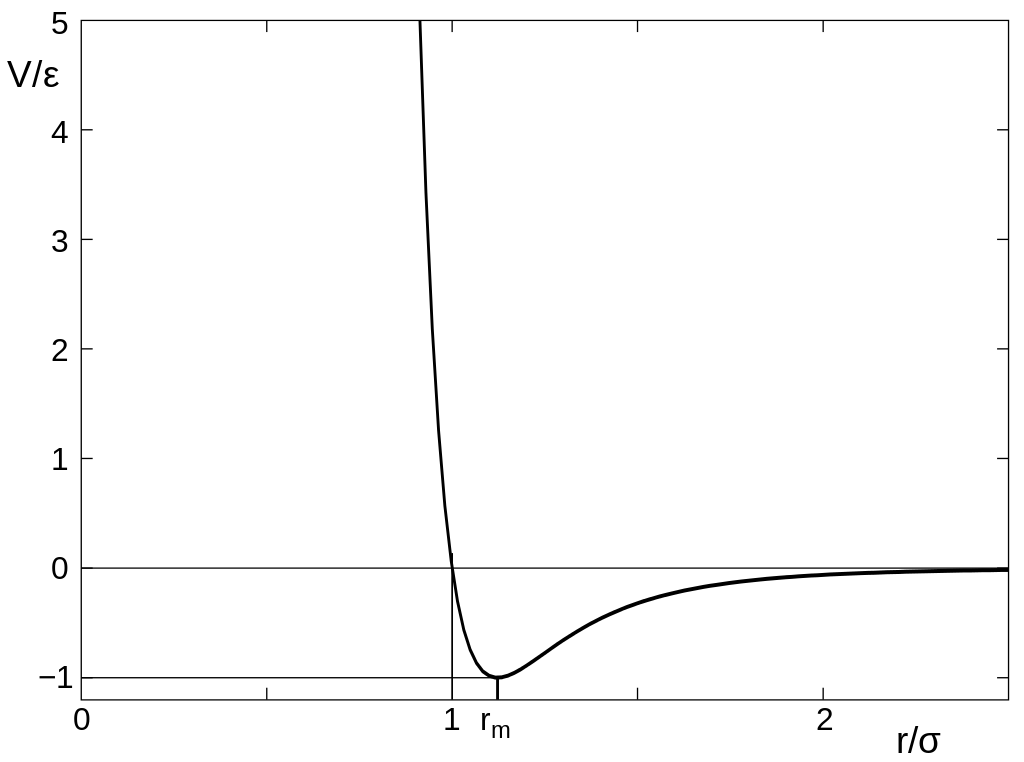
\includegraphics[width=0.8\textwidth, trim=0cm 0cm 0cm 0cm, clip]{MD/figures/lennard_jones.png}
\end{center}
\caption{Da Lennard-Jones potential as a gangbangin' function of relatizzle distizzle $r_{ij}$ between two atoms. (Image from \url{http://en.wikipedia.org/wiki/File:12-6-Lennard-Jones-Potential.svg}, accessed 18 March, 2014.)}
\label{fig:md_lennard_jones}
\end{figure}
With dis potential, we can up in principle calculate tha forces between atoms dat is 10 metas apart. We already know tha answer though, it should be hella, straight-up close ta zero fo' realz. Atoms bein far away from each other do not interact. This distizzle is straight-up not straight-up large. If we bang $r_{ij} = 3.0\sigma$ tha fuck into equation \eqref{eq:md_lj_force}, n' chizzle units so dat $\sigma = \epsilon = 1.0$, we git $F(r=3.0) \approx 0.01$ (compared ta tha maximum attraction near tha potential well $F(r = 1.24) \approx 2.4$, mo' than 100 times larger). Da force decreases slowly towardz zero fo' larger displacements, n' you can put dat on yo' toast. We can exploit dis property n' only compute forces between atoms displaced by a gangbangin' finger-lickin' distizzle smalla than some cut-off radius.
\subsection{Cut-off radius}
\label{sec:md_implementation_two_body_forces}
In principle, we gotta sum over all pairs up in tha system which fo' $N$ atoms is $O(N^2)$. This calculation can be reduced ta $O(N)$ by realizin dat tha gradient of tha potential (hence tha force) is nearly zero at $r \approx 2.5\sigma$. We now introduce tha cut-off radius $r_\text{cut}$, which we chizzle ta be $r_\text{cut} = 2.5\sigma$. Da force between a pair of atoms $F(r_{ij})$ is then freestyled as
\begin{align}
	\vec F(\vec r_{ij}) = \left\{
	\begin{array}{l l}
		-24\epsilon\left[2\left(\frac{\sigma^{12}}{r_{ij}^{13}}\right) - \left(\frac{\sigma^6}{r_{ij}^7}\right)\right]\vec u_{ij} & \text{if } r_{ij} \leq r_\text{cut}\\
		0 & \text{if } r_{ij} > r_\text{cut}.
	\end{array}\right .
\end{align}
This means dat our phat asses don't gotta compute tha forces between atoms dat is mo' than $r_\text{cut}$ apart. Right back up in yo muthafuckin ass. So \textit{locally}, within dis radius $r_\text{cut}$, tha number of pairs we need ta sum over is proportionizzle ta $\rho_n^2$ yo, but if our phat asses double tha system size, most of tha extra atoms do not feel tha forces from tha atoms already up in tha system since they is separated by mo' than $r_\text{cut}$. Right back up in yo muthafuckin ass. So tha calculation of forces is $O(N)$.

We need ta be careful here, cuz tha potential juice is calculated wit tha same rulez all up in tha forces. Right back up in yo muthafuckin ass. So a atom just outside $r_\text{cut}$ gonna git zero potential juice whereas a atom just \textit{inside} gonna git a non-zero juice. This can lead ta erroneous fluctuations up in tha juice. Us thugs will fix dat by shiftin tha potential juice so dat $U(r_\text{cut})$ is zero. Da potential juice is then 
\begin{align}
	U(r_{ij}) = \left\{
	\begin{array}{l l}
		 U_{LJ}(r_{ij}) - U(r_\text{cut}) & \leq r_\text{cut}\\
		0 & \text{if } r_{ij} > r_\text{cut},
	\end{array}\right .
\end{align}
where $U_{LJ}(r_{ij})$ is tha same ol' dirty as up in equation \ref{eq:md_potential_energy}. 